\mysection[black]{5. Optimisation \& Register Alloc.}

\mysubsection{5.1 Optimisation}
\textbf{90/10-Rule}: 90\% of the ex. time is spent in 10\% of the code, mostly loops\\
\textbf{Constant Folding}: If operands are statically known, compute val. and math. simplify: {\scriptsize \texttt{x = (2+3)*y} $\rightarrow$ \texttt{x = 5*y}}\\
\textbf{Const. Prop.}: Prop. var. if c.: {\scriptsize \texttt{x = 5; y = 2*x} $\rightarrow$ \texttt{y = 5*2}}\\
\textbf{Dead Code Elimination (DCE)}: Rem. side-effect free code:  {\scriptsize \texttt{x = y*y; x = z*z} $\rightarrow$ \texttt{x = z*z}} \\
\textbf{Common Subexpression Elimination (CSE)}: Fold redundant comp.:{\scriptsize \texttt{a[i] = a[i] + 1} $\rightarrow$ \texttt{[a + i*4] = [a + i*4] + 1}} \\
\textbf{Strength Reduction}: Replace exp. ops. with cheap ones  {\scriptsize \texttt{loop(a[i*3]=1; ...)} $\rightarrow$ \texttt{i=0; loop(a[i]=1; i=i+3; ...)}}\\
\textbf{Loop Invariant Code Motion (LICM)}: If res. of a expr. doesn't change in loop and it’s pure, can be moved outside body: {\scriptsize \texttt{loop(t=a.length; ...)} $\rightarrow$ \texttt{t=a.length; loop(...)}} \\
\textbf{Loop Unrolling}: Avoid cond. branches:{\scriptsize \texttt{for (int i=0; i<n; i++) \{ S \}} $\rightarrow$ \texttt{i;for (i=0; i<n-3; i+=4) \{S;S;S;S\};for ( ; i<n; i++) \{ S \}}}, unrolling $k$ el. $\frac{k}{k-1}$ branches \\
\textbf{Inlining}: Replace a function call with the body of the function with arguments rewritten to be local variables: pot. renaming var. to avoid naming capture\\
\textbf{Code Specialization}: Create specialized vers. of a fun. that is called from
diff. places with diff. args.\\
\textbf{Speedup[\%]}: $=\left[\frac{\operatorname{base time}}{\operatorname{opt. time}}-1\right]\cdot 100 \%$   



\mysubsection{5.2 Register Allocation}


\textbf{Register Allocation}: Place vars. in same registers if not alive at same time. Reg. much faster than mem.\\
\textbf{Liveness}: \texttt{X} live at \texttt{L} if def. before and used after\\
\textbf{Scoping}: Vars. in diff. scopes are cannot be alive simult.\\
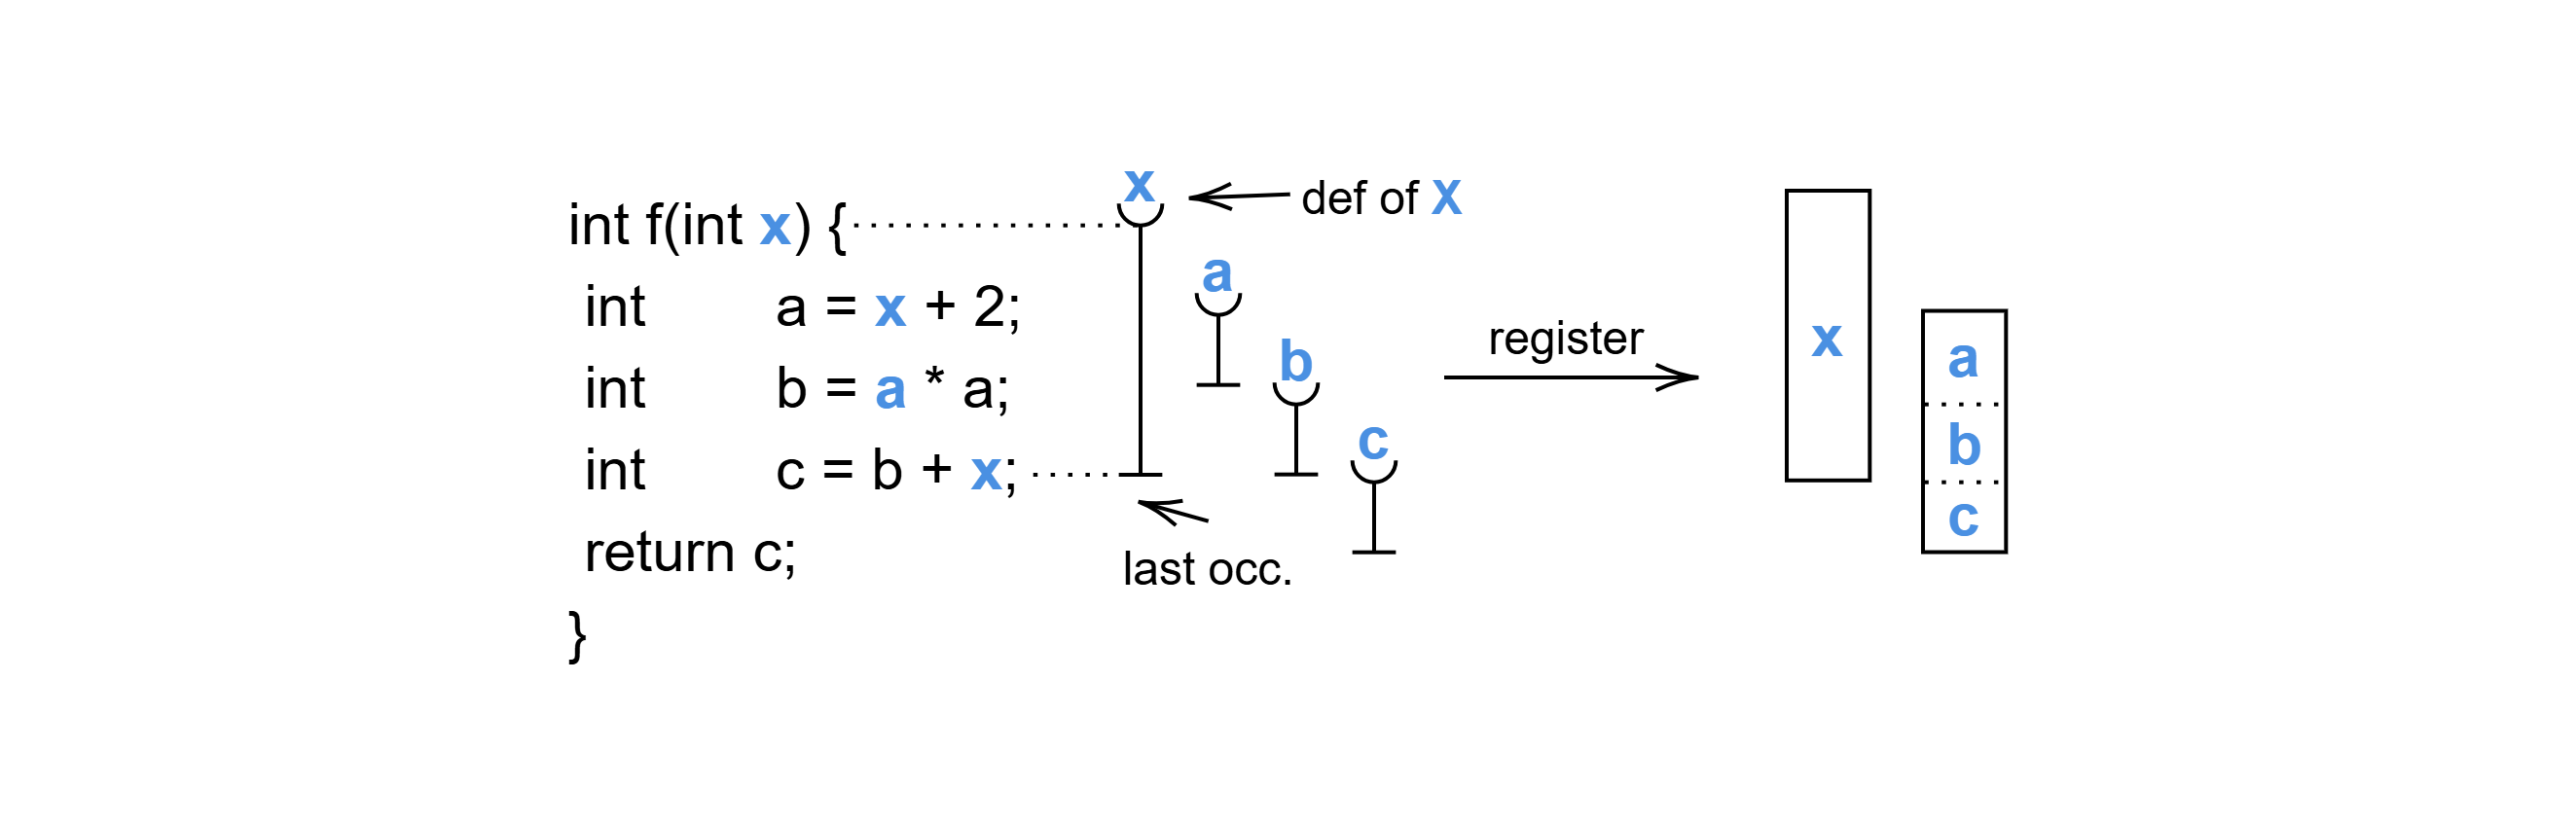
\includegraphics[width=1\linewidth]{images/liveness.png}
\textbf{Alloca Promotion}: Promote stack-allocated variables to SSA registers. Replace alloca + load/store with SSA values and ntroduce $\phi$-nodes where needed\\
\textbf{Stack Spilling}: If not all temps fit into register, spill excess to stack\\
\textbf{Linear-Scan Register Allocation}: 1. Compute set of uids: $\operatorname{live}(x)$ 2. def $\operatorname{pal}$ as usable registers 3. maintain layout by $\operatorname{uid\_loc}$ 4. For each instr. that defines uid $x$: $\operatorname{used} =  \left\{ r \mid \operatorname{reg} r =  \operatorname{uid\_loc}(y) \text{ s.t. } y \in \operatorname{live}(x)\right\}$, $\operatorname{available}= \operatorname{pal} - \operatorname{used}$, if $\operatorname{available}= \emptyset$  then $\operatorname{uid\_loc}= \operatorname{slot}n; n++$ else   $\operatorname{uid\_loc}=\operatorname{reg} r \in \operatorname{available}$, Note that any vars. live over multiple loop iterations are allocated first
\\

\textbf{Graph Coloring}: Compute liveness info for each temp, create interference graph i.e. $E(b_1,b_2)$ iff both are live simult., color graph